\section{ВВЕДЕНИЕ В ИСКУССТВЕННЫЕ НЕЙРОННЫЕ СЕТИ}
Обработка естественного языка является крайне тяжелой задачей для моделирования стандартными алгоритмами. Машинное обучение позволяет решать задачи на основе статистических наблюдений из данных без явной алгоритмизации решения задачи. Недавние прорывы в области обработки естественного языка показывают, что методами машинного обучения можно частично или сполна выполнять многие человеческие задачи, например, краткое изложение текста, написание кода, общение с собеседником и другие, а также добиться результатов распознавания речи сопоставимых с результатами человека \cite{human-wer,whisper}.

Одним из основных аспектов машинного обучения является искусственная нейронная сеть (далее ИНС), созданная по подобию биологических нейронных сетей. Модель ИНС -- описание сети, математическая модель, часто представляемая в виде графа, нацеленная на решение задачи прогнозирования на основе обучающей выборки данных. Методами настройки параметров моделей под конкретную задачу называют методами обучения. Такими методами являются: обучение с учителем, обучение без учителя и обучение с подкреплением.

Каждый метод имеет свои особенности и применяется в зависимости от ситуации. Например, обычно обучение с учителем применяется в тех случаях, когда обучающий набор данных размечен на основе некоторых критериев. Такие задачи обычно являются задачами классификации, когда каждый экземпляр выборки имеет один или больше собственный класс. Такой подход имеет ограничения: как правило количество размеченных данных значительно меньше общего количество данных. В ситуациях, когда данные не размечены, применяется обучение без учителя. Благодаря такому подходу, можно обучить модель делить данные на кластеры, генерировать текст, изображения и т.д. Когда модели приходится принимать решения как интеллектуальный агент в условиях данной ей среды и соотвествующих откликов среды на решения, применяется метод обучения с подкреплением. Для построения мощных современных цифровых ассистенов могут использоваться все три подхода к обучению моделей, используя модели, полученных конкретным методом, в качестве промежуточных или вспомогательных, для обучения конечной модели \cite{state-of-gpt}.

\subsection{УСТРОЙСТВО ПРОСТОЙ ИСКУССТВЕННОЙ НЕЙРОННОЙ СЕТИ}

Устройство простой ИНС можно описать как взвешенный набор узлов, разделенный на слои, соединенные между собой активационными функциями $\varphi$. Функциям активации желательно иметь свойства: нелинейность, непрерывная дифференцируемость, бесконечная область значений, монотонность. При построении модели ИНС в качестве активационных функций часто используется одна из следующих функций:
\begin{enumerate}
    \item Гиперболический тангенс:
          \begin{equation}
              \varphi(z) = \frac{e^{2z}-1}{e^{2z}+1}.
          \end{equation}
    \item Функция ReLU:
          \begin{equation}
              \varphi(z) = \max(0, z).
              \label{relu}
          \end{equation}
    \item Функция GELU:
          \begin{equation}
              \varphi(z) = \frac{1}{2}z\left[1+\text{erf}\left({z}/\sqrt{2}\right)\right].
              \label{gelu}
          \end{equation}
    \item Логистическая функция (сигмоида):
          \begin{equation}
              \varphi(z) = \frac{1}{1+e^{-z}}.
          \end{equation}
    \item Многопеременная логистическая функция (softmax):
          \begin{equation}
              \varphi(z)_i = \frac{e^{z_i}}{\sum_{i=1}^{K}e^{z_j}}.
          \end{equation}
\end{enumerate}

Архитектуры ИНС могут сильно отличаться друг от друга в зависимости от поставленных задач и требований к качеству предсказаний модели. Раздел, который занимается изучением ИНС с большим количеством скрытых слоев, т.е. тех слоев, которые находятся между входным и выходным, называется глубоким обучением, а такие модели называются глубокими. Примером такой архитектуры модели может служить  трансформер \cite{transformer-paper}, речь о котором пойдет дальше.

Набор весов $W$ и отклонений $b$ являются параметрами модели, обозначаемые как $\theta$. Прогноз или функция гипотезы модели ИНС обозначается как $h_{\theta}$. $W^{[l]}$, $b^{[l]}$, $h_{\theta}^{[l]}$ -- веса, отклонения и выход модели на $l$-ом слое. Описать работу обобщенной модели ИНС c $L$ слоями можно следующим образом:
\begin{enumerate}
    \item $h_{\theta}^{[0]} = x$.
    \item $h_{\theta}^{[l]} = \varphi \circ \left(W^{[l-1]}h_{\theta}^{[l-1]}(x) + b^{[l-1]}\right), \text{где } 1 \le l \le L-1$.
    \item $h_{\theta} = h_{\theta}^{[L]} = W^{[L-1]}h_{\theta}^{[L-1]}(x) + b^{[L-1]}$.
\end{enumerate}

Примером простой ИНС может являться однослойный перцептрон. Схема однослойного перцептрона представлена на рис. \ref{fig:perceptron}.

\begin{figure}[H]
    \centering
    \begin{tikzpicture}[
            init/.style={
                    draw,
                    circle,
                    inner sep=2pt,
                    font=\Huge,
                    join = by -latex
                },
            squa/.style={
                    draw,
                    inner sep=2pt,
                    font=\Large,
                    join = by -latex
                },
            start chain=2,node distance=17mm
        ]
        \node[on chain=2]
        (x2) {$x_2$};
        \node[on chain=2,join=by o-latex]
        {$w_2$};
        \node[on chain=2,init] (sigma)
        {$\displaystyle\Sigma$};
        \node[on chain=2,squa,label=above:{\parbox{2cm}{\centering Функция \\ активации}}]
        {$\varphi$};
        \node[on chain=2,label=above:Выход,join=by -latex]
        {$y$};
        \begin{scope}[start chain=1]
            \node[on chain=1] at (0,1.5cm)
            (x1) {$x_1$};
            \node[on chain=1,join=by o-latex]
            (w1) {$w_1$};
        \end{scope}
        \begin{scope}[start chain=3]
            \node[on chain=3] at (0,-1.5cm)
            (x3) {$x_3$};
            \node[on chain=3,label=below:Веса,join=by o-latex]
            (w3) {$w_3$};
        \end{scope}
        \node[label=above:\parbox{2cm}{\centering Отклонение\\$b$}] at (sigma|-w1) (b) {};

        \draw[-latex] (w1) -- (sigma);
        \draw[-latex] (w3) -- (sigma);
        \draw[o-latex] (b) -- (sigma);

        \draw[decorate,decoration={brace,mirror}] (x1.north west) -- node[left=10pt] {Вход} (x3.south west);
    \end{tikzpicture}
    \caption{Однослойный перцептрон}
    \label{fig:perceptron}
\end{figure}

\subsection{ОБУЧЕНИЕ С УЧИТЕЛЕМ ИСКУССТВЕННОЙ НЕЙРОННОЙ СЕТИ}

Как было сказано раннее, для того, чтобы обучить ИНС с учителем, требуется иметь такой набор данных, где каждый элемент имел соответствующую метку класса. Элементы набора данных, т.е. входные данные, принадлежат некоторому входному пространству $\mathcal{X}$, например, картинкам кошек, а метки принадлежат к выходному пространству $\mathcal{Y}$, например, породе кошек. Из такого набора данных $\mathcal{D}$ мы строим тренировочную подвыборку, состоящую из пар, элементов:

\begin{equation}
    \mathcal{D}_{\text{train}} = \{\,(x_i, \hat y_i) \mid x_i \in \mathcal{X}, \hat y_i \in \mathcal{Y}, i=\overline{1, \dots, n}, n \le \lvert \mathcal{D} \rvert\,\}.
\end{equation}

Мы стремимся получить целевую функцию ИНС $h_{\theta^*}$ с оптимальным набором параметров $\theta^*$ на основе $\mathcal{D}_{\text{train}}$, при котором $h_{\theta^*}$ наиболее эффективно отображает из пространства $\mathcal{X}$ в пространство $\mathcal{Y}$. Для определения того, насколько эффективно предсказывает модель, требуется иметь неотрицательную функцию $\ell: \mathcal{Y} \times \mathcal{Y} \rightarrow \mathbb{R}^+$, которая измеряет ошибку предсказания $h_{\theta}(x)$ по отношению к истинной метке $\hat y$. Такие функции, как правило, называются функциями ошибки или функциями потерь. Функция потерь выбирается исходя из условий конкретной задачи, но часто является одной из следующих функций:
\begin{enumerate}
    \item Функция потерь $L_1$:
          \begin{equation}
              \ell\left(h_\theta(x), \hat y\right) = \lvert \hat y - h_\theta(x) \rvert.
          \end{equation}
    \item Функция потерь $L_2$:
          \begin{equation}
              \ell\left(h_\theta(x), \hat y\right) = \big(\hat y - h_\theta(x)\big)^2.
          \end{equation}
    \item Функция потерь перекрестной энтропии:
          \begin{equation}
              \ell\left(h_\theta(x), \hat y\right) = - \hat y\log{h_\theta(x)}.
          \end{equation}
    \item Функция потерь NLL:
          \begin{equation}
              \ell\left(h_\theta(x), \hat y\right) = -\left[\hat y \log{h_\theta(x)} + (1 - \hat y)\log(1 - h_\theta(x))\right].
          \end{equation}
\end{enumerate}

Обучение модели с учителем сводится к задаче минимизации функции потерь по тренировочной выборке:

\begin{equation}
    \mathcal{L}_{\mathcal{D}_{\text{train}}}(\theta) = \frac{1}{\lvert \mathcal{D}_{\text{train}} \rvert}\sum_{i=1}^{\lvert \mathcal{D}_{\text{train}} \rvert}\ell(h_{\theta}(x_i),\hat y_i) \rightarrow \min_{\theta}.
\end{equation}

Чтобы решить такую задачу минимизации функции потерь по тренировочной выборке, требуется вычислить:

\begin{equation}
    \frac{\partial \mathcal{L}_{\mathcal{D}_{\text{train}}}(\theta)}{\partial \theta}.
    \label{loss-grad}
\end{equation}

Метод, который позволяет аналитически вычислить градиент (\ref{loss-grad}) в точке, называется методом обратного распостранения ошибки \cite{backprop-theory}. Основа метода -- автоматическое построение графа вычислений и правило вычисления производной сложной функции. С полученным градиентом функции потерь параметры модели ИНС меняются алгоритмом оптимизации. Одними из важных составляющих алгоритмов оптимизации являются выбор размера шага оптимизатора $\eta$, называемым еще скоростью обучения, и планировщик скорости обучения $\varsigma$, поскольку влияют на скорость процесса обучения и на преодоления методом оптимизации локальных минимумов. Частым выбором таких алгоритмов являются: <<\textit{GD}>> (градиентный спуск), <<\textit{SGD}>> (стохастический градиентный спуск), Adam, AdaFactor \cite{optimizers-paper,adafactor-paper}.

Обучение является итеративным процессом, где итерация или шаг итерации -- это обработка моделью одного или нескольких примеров обучающей выборки. Обработка полного набора выборки называют эпохой.

Алгоритм обучения модели ИНС с учителем представлен ниже.

\begin{algorithm}
    \floatname{algorithm}{Алгоритм}
    \caption{Обучение модели ИНС с учителем}
    \begin{algorithmic}[1]
        \State Инициализировать $\theta$ случайно или по некоторому закону распределения.
        \State По каждой эпохе из количества эпох:
        \State\hspace{\algorithmicindent} По каждому примеру $(x, \hat y)$ из обучающей выборки $\mathcal{D}_{\text{train}}$:
        \State\hspace{\algorithmicindent}\hspace{\algorithmicindent} Получить предсказание модели $y \gets h_{\theta}(x)$.
        \State\hspace{\algorithmicindent}\hspace{\algorithmicindent} Получить значение функции потерь $\ell(y, \hat y)$.
        \State\hspace{\algorithmicindent}\hspace{\algorithmicindent} Получить градиент $\nabla \ell$ методом обратного распостранения.
        \State\hspace{\algorithmicindent}\hspace{\algorithmicindent} Сделать шаг оптимизации.
        \State\hspace{\algorithmicindent}\hspace{\algorithmicindent} Аккумулировать значение общей функции потерь $\mathcal{L} \gets \mathcal{L} + \ell(y, \hat y)$.
    \end{algorithmic}
\end{algorithm}

Однако одной тренировочной подвыборки чаще всего не достаточно для успешного обучения модели. Как правило используют три подвыборки исходных данных $\mathcal{D}$. Помимо обучающей, используется валидационная $\mathcal{D}_{\text{val}}$, которая используется в конце эпохи обучения, на которой модель не обучается, но проверяется на наборе данных, которые она не видела, для корректировки гиперпараметров модели. Гиперпараметры -- это параметры, которые используются для контроля процесса обучения. Примерами гиперпараметров могут служить как вышеупомянутые $\eta$ и $\varsigma$, так и количество слоев в модели, активационные функции и т.д. Для оценки итогого качества модели обычно используется тестовая выборка $\mathcal{D}_{\text{test}}$. Методы, которые разбивают исходный набор данных $\mathcal{D}$ на подвыборки, называются методами стратификации.

Хоть $\ell$, $\mathcal{L}$ и показывают качество прогнозирования модели $h_{\theta}$, но на практике анализировать качество модели только по значениям функции потерь -- это сложная задача. Помимо функции потерь используются метрики оценки прогнозирования. Выбор метрик сильно зависит от поставленной задачи.

\section{ВЕКТОРНОЕ ПРЕДСТАВЛЕНИЕ ТЕКСТА}
Из устройства работы ИНС следует, чтобы данные, на которых обучается модель были численными. Поэтому при обработке текста требуется получить его векторное представление для дальнейшей работы с ним.

Простейшим методом представления слов в векторном пространстве является <<\textit{One-Hot Encoding}>> (быстрое кодирование). Его суть заключается в присвоении каждому слову из входной последовательности слов вектора, где в позиции, соотвествующей слову в словаре размерностью словаря, ставится единица, а во всех остальных позициях -- ноль. Словарь содержит весь список возможных слов для кодирования. Размерность такого вектора составляет $1 \times N$, где $N$ -- количество слов в словаре. Пример быстрого кодирования показан ниже.

\begin{table}[H]
    \captionsetup{format=hang, singlelinecheck=false}
    \raggedleft
    \caption{Пример словаря}
    \label{tab:dict}
    \centering
    \begin{tabular}{|p{5cm}|}
        \hline
        \textbf{Цвет} \\
        \hline
        Красный       \\
        \hline
        Зеленый       \\
        \hline
        Синий         \\
        \hline
    \end{tabular}
\end{table}

\begin{table}[H]
    \captionsetup{format=hang, singlelinecheck=false}
    \raggedleft
    \caption{Пример быстрого кодирования}
    \label{tab:ohe}
    \centering
    \begin{tabular}{|p{5cm}|p{5cm}|p{5cm}|}
        \hline
        \textbf{Красный} & \textbf{Зеленый} & \textbf{Синий} \\
        \hline
        1                & 0                & 0              \\
        \hline
        0                & 1                & 0              \\
        \hline
        0                & 0                & 1              \\
        \hline
    \end{tabular}
\end{table}

Представлением текстовых данных в численном виде могут заниматься и модели ИНС: учить полезную информацию о входной последовательности, сжато представлять текст в векторном пространстве, решая задачу языкового моделирования, для последующего использования этого представление на конечной задаче, например, задаче классификации или задаче генерации текста. Одной из первых широко распостраненных обученных моделей для кодирования текста является Word2vec \cite{word2vec-paper}.

В современных моделях для обработки естественного языка в качестве основы векторного представления данных используют метод, называемый токенизацией. Токенизация -- разбиение входного текста на части, называемые токенами. В качестве части текста могут быть как слова целиком, так и части слов. Токенизация представляет входной текст как вектор, состоящий из номеров токенов в общем словаре. Размер закодированной последовательности может зависеть как длиной входной последовательности, так и от требуемой длины, дополняя неиспользуемое пространство специальными токенами. Пример токенизации <<\textit{Byte-Pair Encoding}>> (побайтное кодирование) \cite{bpe-paper} для входной последовательности <<Many words map to one token, but some don't: indivisible. Sequences of characters commonly found next to each other may be grouped together: 1234567890>> представлен ниже. Токены, на которые разбивает токенизитор входную последовательность, показаны на рис. \ref{fig:tok-viz-words-fig}.
\begin{figure}[H]
    \centering
    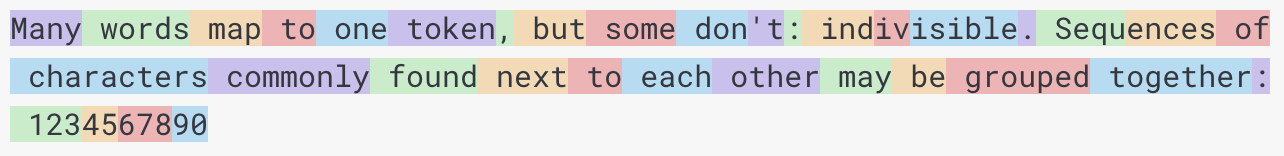
\includegraphics[width=\textwidth]{tok-viz-words-fig}
    \caption{Пример работы токенизации}
    \label{fig:tok-viz-words-fig}
\end{figure}

Векторное представление такой последовательность токенов показано на рис. \ref{fig:tok-vec}.
\begin{figure}[H]
    \centering
    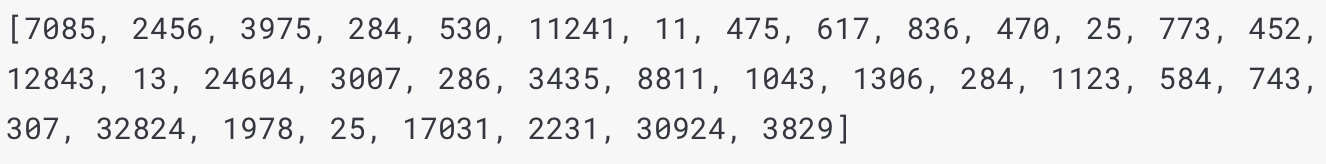
\includegraphics[width=\textwidth]{tok-vec}
    \caption{Векторное представление токенов}
    \label{fig:tok-vec}
\end{figure}

\section{АРХИТЕКТУРА ТРАНСФОРМЕР}
Стандартным выбором архитектуры модели ИНС при обработке естественного языка является архитектура трансформер. Одними из первых моделей, созданных на базе данной архитектуры, стали GPT \cite{gpt-paper}, T5 \cite{t5-paper} и BERT \cite{bert-paper}. Трансформер состоит из набора блоков <<\textit{encoder}>> (кодировщика) и <<\textit{decoder}>> (декодировщика).

Для начала происходит токенизация входного текста, а затем полученное векторное представление токенов дополняется позициональным кодированием, чтобы учитывать информацию о позиции токена во входном тексте.

Далее полученное векторное состояние передается на $N$ идущих друг за другом блоков кодировщика. Каждый блок кодировщика состоит из двух главных компонент: механизм <<\textit{Self-Attention}>> (самовнимание) и сети прямого распостранения (обобщенная версия сети, показаной на рис. \ref{fig:perceptron}). После прохождения $N$ блоков кодировщика, векторное состояние передается к $N$ блокам декодировщика.

В свою очередь каждый блок декодировщика схож с устройством блока кодировщика с добавлением <<\textit{Cross-Attention}>> (перекресного внимания) от векторного представления состояния кодировщика. Полную версию архитектуры трансформер можно наблюдать на рис. \ref{fig:transformer-arch}.
\begin{figure}[H]
    \centering
    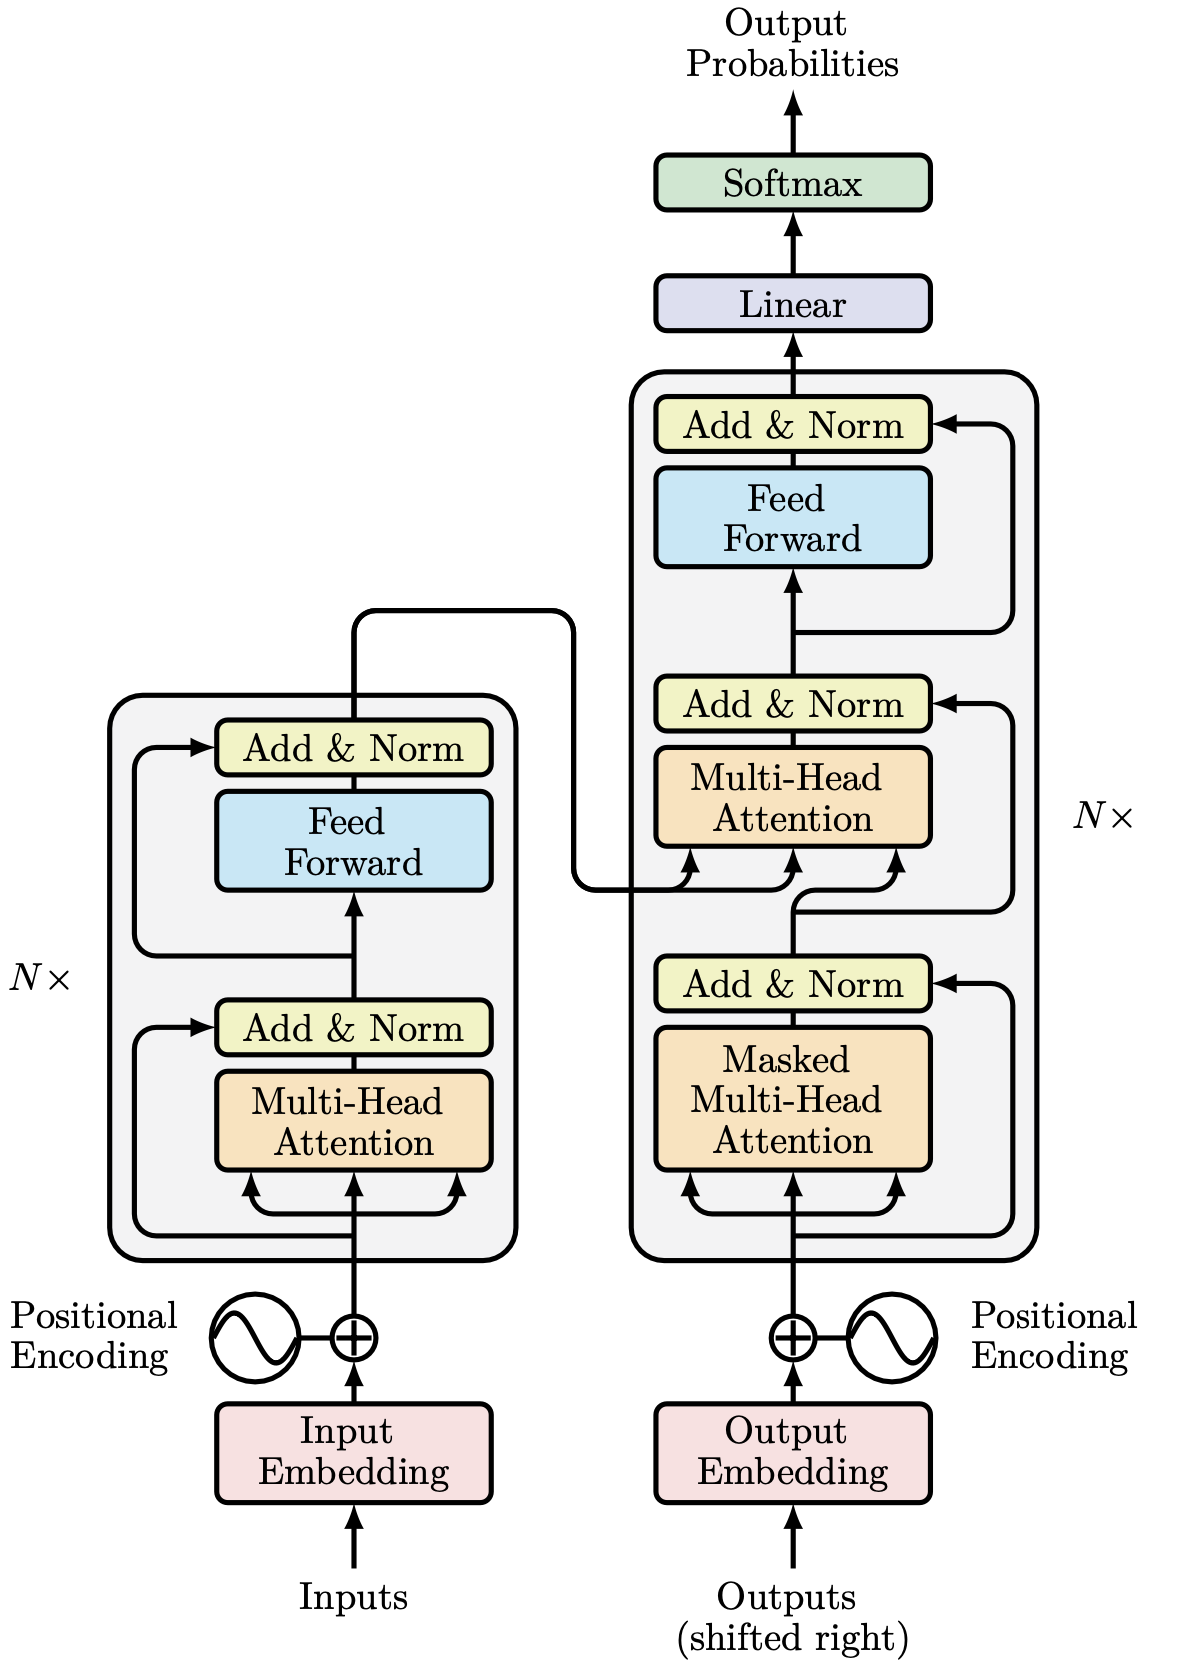
\includegraphics[width=0.55\textwidth]{transformer-arch}
    \caption{Архитектура трансформер}
    \label{fig:transformer-arch}
\end{figure}
\subsection{МЕХАНИЗМ ВНИМАНИЯ}
Механизм внимания -- ключевой механизм в архитектуре трансформер. Его суть заключается в учитывании взаимодействия элемента входной последовательности со всеми другими элементами. Таким образом, модель может фокусироваться на более важных частях данных, даже если такая информация содержится в небольшой части данных.

Разберем более подбробно этот механизм. Входное векторное состояние данных представляется как набор трех главных компонент внимания: <<\textit{query}>> (запрос), <<\textit{keys}>> (ключи) и <<\textit{values}>> (значения). Преставление входных данных осуществляется за счет проекции входного векторного состояния $I$ на пространства этих компонент, т.е.:

\begin{enumerate}
    \item $Q = I \cdot W_Q^T$.
    \item $K = I \cdot W_K^T$.
    \item $V = I \cdot W_V^T$.
\end{enumerate}

Из полученных векторов вычисляем результирующий вектор:

\begin{equation}
    \text{Attention}\left(Q,K,V\right) = \text{softmax}\left(\frac{QK^T}{\sqrt{d_k}}\right)V\text{, где }d_k = \dim(K).
    \label{eq:attn}
\end{equation}

Проинтерпретировать формулу \ref{eq:attn} можно следующим образом:

\begin{enumerate}
    \item Запрос $Q$ проектируется в пространство ключей $K$, т.е. получаем матрицу: $S = QK^T$.
    \item Для запроса $Q$ в смаштабированном пространстве $K$ ищется наиболее подходящие, т.е. близкие ключи: $A=\text{softmax}\left(\frac{S}{\sqrt{d_k}}\right)$.
    \item Затем полученная матрица умножается на искомые значения, получая взвешенную сумму входного векторного состояния: $O=AV$.
\end{enumerate}

Важно отметить, что матрицы внутренного состояния $W_Q,W_K,W_V$ -- обучаемые параметры.

В случае, когда $Q, K, V$ получаются из одного внутреннего состояния, такой вид механизма внимания называется самовнимание. Если $K, V$ получены как выход внутреннего состояния кодировщика, а $Q$ получен как внутренне состояние декодировщика, то такой вид внимания называется перекресным вниманием. Такой механизм позволяет модели учитывать взаимодействие между элементами входной и выходной последовательностей. Таким образом, блоки декодировщика могут использовать информацию из блоков кодировщика для генерации правильных элементов выходной последовательности.

Также может потребоваться, чтобы модель оперировала векторным состоянием входного текста до позииции текущего токена. Чтобы закрыть доступ модели к такого рода информации, применяется маскированное внимание.

Вместо вычисления одного внимания с размерностью $d_{\text{model}}$, можно вычислять внимание c фокусом на разные участки входной последовательности параллельно. Такое внимание называется <<\textit{Multi-Head Attention}>> (многоголовое внимание) и вычисляется как:

\begin{equation}
    \text{MHA}(Q, K, V) = \text{Concat}(\text{head}_1, \dots, \text{head}_h) W^O,
\end{equation}

где $\text{head}_i = \text{Attention}(QW_i^Q, KW_i^K, VW_i^V)$.

Благодаря тому, что операции перемножения матриц -- высокооптизируемые операции, данный механизм эффективен с точки зрения производительности.

\subsection{МОДЕЛЬ T5: АРХИТЕКТУРА И ЕЕ ОСОБЕННОСТИ}
Обучение модели архитектуры трансформер обычно происходит в два этапа. Сначала модель обучается решать задачу языкового моделирования на огромном наборе неразмеченных данных. Такой процесс крайне затратен, т.к. требует больших мощностей и огромного набора данных. Такой этап называется <<\textit{pretrain}>> (предварительное обучение), после чего модель дообучают на конкретной задаче, например, на генерации текста или на задаче поддержания диалога, на меньшем, но размеченном наборе данных. Этап дообучения значительно менее затратен, чем предварительное обучение.

Модель <<\textit{Text-To-Text Transfer Transformer}>> (T5) -- это модель глубокого обучения, использующая архитектуру трансформер, разработанная компанией Google для решения многих различных задач обработки естественного языка. Преимущества данной модели является универсальность: Т5 изначально была обучена на задачах перевода, кратком изложении текста, классификации текста и на ответа на вопрос, разделяя задачи специальным префиксом. Одной из особенностей моделей T5 является их способность работать с разными типами входных и выходных данных. Например, модель может обрабатывать текстовые данные различных длин и форматов, а также генерировать тексты различных стилей и тематик. В качестве токенизатора T5 использует SentencePiece \cite{sentencepiece-paper}.

Предварительное обучение Т5 производилось на наборе данных <<\textit{Colossal Clean Crawled Corpus}>> (C4), содержащий 356 миллиардов токенов, занимающий 750Гб дискового пространства, на задаче <<\textit{Masked Language Modeling}>> (моделирование замаскированного языка). Задача заключается в востановлении исходного текста на основе <<поврежденного>> текста, где <<повреждалось>> 15\% токенов, в которых 90\% заменялось на специальный токен \texttt{[MASK]}, а остальные 10\% заменялись на случайный токен из словаря.

После предварительного обучения модель дообучили на конечных задачах, описанных выше. Со временем набор изначальных задач расширили набором задач, состоящим из инструкций на понимание и генерацию текста на естественном языка, что значительно улучшило качество модели для последующего обучения, например, на задаче поддержания диалога \cite{flan-paper}.

\section{ПОСТАНОВКА ЗАДАЧИ ДИАЛОГОВОЙ СИСТЕМЫ}
Эмуляция диалога, обучение диалоговых агентов или чат-ботов относятся к области генерации и классификации текста. Такие модели должны эффективно обрабатывать естественный язык и формировать ответы в рамках диалога. В качестве диалоговой системы может выступать не одна модель ИНС. Различные задачи, например, классификации, генерации текста и автоматичского распознавания речи могут выполнять разные модели. Разберем основные компоненты диалога:

\begin{enumerate}
    \item Состояние диалога: Диалоговая система должна понимать намерения запроса пользователя и те сущности, которые фигурируют в запросе. Намерением пользователя может быть покупка, а сущностью -- товар. Такие задачи являются задачами классификации.
    \item Контекст диалога: диалоговая система должен учитывать контекст предыдущих сообщений, чтобы дать более точный и подходящий ответ.
    \item Цель диалога: диалоговая система может иметь цель, которую она преследует в рамках диалога. Такой целью может быть, например, имитация поведения неигрового персонажа.
    \item Шаг диалога: одна итерация в обмене сообщениями между пользователем и диалоговой системой. Каждый шаг диалога представляет собой один вопрос или одно сообщение от системы, на которое пользователь должен ответить. Затем система обрабатывает ответ пользователя и переходит к следующему шагу диалога. Шаги диалога помогают упорядочить и структурировать обмен сообщениями между пользователем и диалоговой системой. Пример шагов диалога приведет в таблице \ref{tab:dialogue-turn}.
\end{enumerate}

\begin{table}[H]
    \captionsetup{format=hang, singlelinecheck=false}
    \raggedleft
    \caption{Пример диалоговых шагов}
    \label{tab:dialogue-turn}
    \centering
    \begin{tabular}{|p{5cm}|p{10cm}|}
        \hline
        Шаг 1 & Система: Здравствуйте, чем я могу Вам помочь?            \\
        \hline
        Шаг 2 & Пользователь: Добрый день, я хочу заказать пиццу на дом. \\
        \hline
        Шаг 3 & Система: Какой размер пиццы Вы хотели бы заказать?       \\
        \hline
    \end{tabular}
\end{table}

Для обучения диалоговых моделей, способных продолжить диалог, требуется набор данных, содержащий диалоги. Такую задачу можно решить обучением с учителем. Для этого необходимые компоненты диалога должны быть в формате $(x, \hat y)$, где в качестве $x$ выступает строка, содержащая цель диалога и его контекст, а в качестве $\hat y$ выступает желаемый ответ диалоговой модели.